\section{Research}
\label{sec:research}

An introduction of the research, including the main research question, is presented in \cref{sec:introduction}. \Cref{sec:focus} describes more details of the research and the sub-problems. In \cref{sec:paper}, a list of resulted papers and reports is shown. \Cref{sec:outlook} provides an outlook for the coming years of my PhD.


\subsection{Introduction}
\label{sec:introduction}

% Automated Vehicles are introduced (in Singapore)
The development of automated vehicles (AVs) has made significant progress. It is expected that before 2020, automated and autonomous vehicles will be introduced in controlled environments, whereas autonomous vehicles will be mainstream by 2040 \cite{madni2018autonomous} or earlier \cite{bimbraw2015autonomous}. Especially in densely populated cities such as Singapore, there is a need for automated vehicles to increase traffic safety and traffic efficiency by enabling flexible, automated, mobility-on-demand systems \cite{spieser2014toward}, scheduled services for public transport needs, and automated freight and service vehicles to support 24 hours operations and labor shortage needs.

% Assessment of AVs is important
An important aspect in the development of AVs is the safety assessment of the AVs \cite{bengler2014threedecades, stellet2015taxonomy, putz2017pegasus, wachenfeld2016release}. For legal and public acceptance of AVs, a clear definition of system performance is important, as are quantitative measures for the system quality. The more traditional methods \cite{ISO26262, response2006code}, used for evaluation of driver assistance systems, are no longer sufficient for assessment of the safety of higher level AVs, as it is not feasible to complete the quantity of testing required by these methodologies \cite{wachenfeld2016release}. Therefore, the development of assessment methods is important to not delay the deployment of AVs \cite{bengler2014threedecades}.

% Scenario-based approach
One proposed way to assess safety is to test drive AVs in real traffic, observe their performance, and make statistical comparisons to human driver performance. However, this requires AVs to drive hundreds of millions of kilometers and sometimes hundreds of billions of kilometers to demonstrate their reliability in terms of fatalities and injuries \cite{kalra2016driving}. It does not seem to be feasible to drive these millions of kilometers with the increased speed of development of automated driving (AD) functions and the high level of safety requirements that are expected from these functions. As an alternative, a scenario-based assessment is adopted \cite{putz2017pegasus, stellet2015taxonomy, deGelder2017assessment, ploeg2018cetran, elrofai2018scenario}. 
% Scenarios are obtained with data
These test-scenarios can be knowledge-driven or data-driven \cite{stellet2015taxonomy}. A drawback of knowledge-based test scenarios is that it does not allow to generalize the results to the performance of the system-under-test when operating in traffic, i.e., the test cases may not be valid or representative for real-world traffic. A data-driven approach is adopted, as it allows to generalize the results \cite{deGelder2017assessment}. The challenge is, however, to extract the interesting, e.g., performance critical, scenarios from the data, such that the number of simulations is still limited.

In summary, the ultimate goal of this research is a methodology for generating test case that assess the performance of an AV using a data-driven approach. Hence, the main research question is formulated as follows:

\begin{mdframed}[style=MyFrame]
	\paragraph{Main research question:} How can test cases be generated that assess the performance of automated vehicles in real traffic using real-world driving data?
\end{mdframed}

\subsection{Focus of research}
\label{sec:focus}

\Cref{fig:scheme} presents a schematic overview of the process of the assessment of an automated vehicle using real-world driving data. The primary goal of the research is to develop a methodology for the generation of the test cases using the preprocessed data, represented by the green blocks in \cref{fig:scheme}. This is achieved by detecting and parameterizing so-called activities. Using the activities and the static environment, the scenarios can be obtained, after which test cases can be generated for the assessment of the AV.

\tikzstyle{block}=[node distance=5.2em, text width=4.5em, minimum height=7em, align=center, rounded corners=8pt, font=\small]
\tikzstyle{my brace}=[decorate, decoration={brace, amplitude=10pt}]
\tikzstyle{horz}=[node distance=2.7em]
\tikzstyle{vert}=[node distance=4em]
\begin{figure}[b]
	\centering
	\begin{tikzpicture}[scale=0.95, every node/.style={transform shape}]
		% Draw the blocks
		\node[block, fill=blue!30](dc){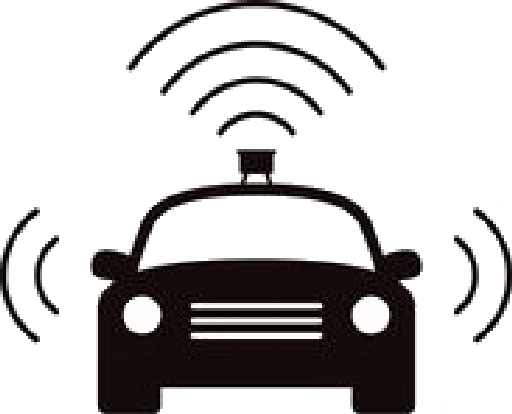
\includegraphics[width=4em]{data_collection.png} \\ Data collection};
		\node[block, fill=blue!30, right of=dc](dp){
\includegraphics[width=2.5em]{data_processing.png} \\ Data preprocessing};
		\node[block, fill=green!30, right of=dp](ed){
\includegraphics[width=4.2em]{event_detection.png} \\ Activity detection};
		\node[block, fill=green!30, right of=ed](s){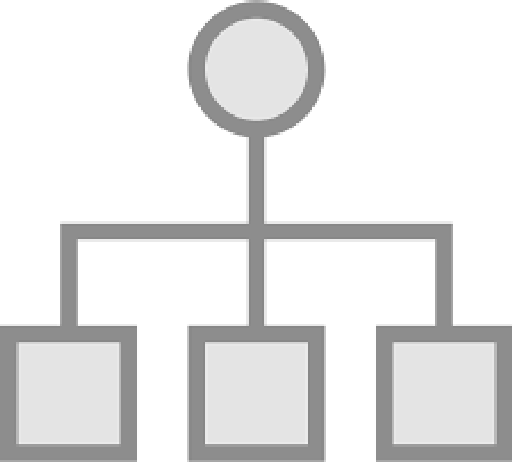
\includegraphics[width=3em]{scenario_mining.png} \\ Scenario mining};
		\node[block, fill=green!30, right of=s](p){
\includegraphics[width=3em]{parametrisation.png} \\ Parame-trization};
		\node[block, fill=green!30, right of=p](tc){
\includegraphics[width=3.2em]{scenarios.png} \\ Test case genera-tion};
		\node[block, fill=red!30, right of=tc](sim){
\includegraphics[width=4em]{simulation.png} \\ Simulation};
		\node[block, fill=red!30, right of=sim](eval){
\includegraphics[width=3em]{evaluation.png} \\ Evaluation};
		
		% Show completeness part
		\node[horz, left of=ed](b1){};
		\node[vert, below of=b1](b2){};
		\node[horz, right of=tc](b3){};
		\node[vert, below of=b3](b4){};
		\draw[my brace](b4) -- (b2) node[midway, yshift=-2em, align=center]{Completeness};
	\end{tikzpicture}
	\vspace{-1em}
	\caption{Schematic overview of the process of the assessment of an automated vehicle using real-world data. The green blocks are the focus of the PhD research.}
	\label{fig:scheme}
\end{figure}


% Definition of scenario
First of all, a clear definition of scenario is required to avoid the ambiguity that often arises when talking about \emph{scenarios}. Next to that, related notions need to be defined, e.g., the components that constitute a scenario, such as the activities and the static environment. The goal is to formally define scenario and the related notions, such that these definitions can be directly reflected to, e.g., code and database structure.

% Activity detection
An activity is considered the smallest building block of the dynamic part of the scenario (maneuver of the ego vehicle and the dynamic environment). An activity refers to the behavior of an actor, such as ``braking'' and ``changing lane''. The first step is to detect the activities from the preprocessed data. 

% Scenario mining
In scenario mining, the events and activities that are independently identified for the ego vehicle, the other traffic participants, the static environment, and the conditions are combined to construct a scenario. 

% Parametrization
The recorded scenarios (and its associated activities) are to be stored in a database \cite{elrofai2018scenario}. The scenario database does not contain raw sensor data, but a parametrized model of the real world based on the sensor signals. Therefore, dependency of the stored scenarios on the sensor set with which the scenario was recorded is avoided. The fact that the stored scenarios do not contain the original sensor data brings several benefits: 
\begin{itemize}
	\item The original sensor data might be sensitive as it reveals the sensor setup and processing capabilities of a car. This is much less of an issue when only parameters of the models of the scenarios are stored. Whereas the original sensor data is unlikely to be shared among different parties, the resulting scenarios might be shared, such that the involved parties can benefit from each other.
	\item By condensing the information of all sensors into the least number of parameters that describe the scenario within the error bounds of sensors, substantial reduction in storage volume is achieved.
	\item All the parameters of scenarios of a specific scenario class can be used to construct probability density functions. These probability density functions can be used to generate test cases that lead to probabilistic results \cite{deGelder2017assessment}. Furthermore, it is possible, using the parametrized scenarios, to emphasize scenarios in which the system-under-test shows performance-critical behavior without a-priori knowledge of what scenarios might be critical \cite{deGelder2017assessment}. 
	\item The parametrized models of the scenarios allow for time interpolation. Hence, the stored scenarios can be used for any given sample time, regardless of the sample time of the original sensor data. 
\end{itemize}

% Test case generation
To generate the test cases, the parametrized scenarios are used. More specifically, a probability density function (pdf) of the parameters is estimated. By drawing samples from the pdf, new test cases are generated. The parametrization influences the estimation of the pdf, e.g., the number of parameters and the correlation among the parameters influence the uncertainty of the estimation. In general, the test case generation will be easier when fewer parameters are used to describe a scenario. On the other hand, using too few parameters might result in a loss of important information of the scenario. It needs to be investigated what the balance is between having enough parameters to retain sufficient information while enabling reliable generation of test cases.

% Completeness
On the one hand, the number of scenarios should be limited such that the test load remains feasible and, on the other hand, the scenarios should cover a large part of the variety of the actual scenarios that can be found in real-world traffic. For this reason, it is important to quantify to what extent the collected scenarios and the test cases are \emph{complete}. In \cref{fig:scheme}, this is indicated by the notion of \emph{completeness}. A goal of this research is to quantify the \emph{completeness} of the data.

% Research question
Based on the main research question, many sub-questions can be formulated. To limit the scope of the research, only three sub-questions are formulated. 

\begin{mdframed}[style=MyFrame]
	\paragraph{Sub-question 1:} How to formally define scenario in the context of the assessment of automated vehicles?
	
	\paragraph{Sub-question 2:} How to parametrize scenarios while retaining sufficient information and enabling reliable estimation of the probability density function of the parameters?
	
	\paragraph{Sub-question 3:} How to quantify the completeness of the driving data?
\end{mdframed}

Some preliminary results regarding sub-questions 1 and 3 are presented in \cref{sec:results}.

\subsection{Papers and reports}
\label{sec:paper}

During last year, several papers and reports are written, among which are the following:
\begin{enumerate}
	\item Paper on ontology for scenarios, see \cref{sec:attached papers}, submitted to the Intelligent Vehicles Symposium (IV). Unfortunately, the paper has been rejected. The main criticism was that the paper presents a set of definitions, rather than an ontology.
	\item When working at CETRAN, I worked on a report that describes the framework for the scenario-based assessment of AVs. Part of this report has been turned into a paper for the Intelligent Transportation Systems (ITS) Asia-Pacific Forum \cite{ploeg2018cetran} of which I am the second author, see \cref{sec:attached papers}.
	\item Together with Olaf Op den Camp, I wrote a report describing different scenario classes relevant for Singaporean traffic. To do this, use is made of the ontology defined earlier, so this report might be a good use case of the ontology. We aim to have this document publicly available as soon as it is finalized. \label{item:scenario classes}
	\item The methodology of generating test cases for the assessment of AVs using real-world driving data is called ``StreetWise'' within TNO. TNO wrote a position paper on this topic \cite{elrofai2018scenario}.
\end{enumerate}

\subsection{Outlook}
\label{sec:outlook}

My goal is to write at least four journal papers on the following topics:
\begin{itemize}
	\item \emph{Ontology for scenarios for the assessment of AVs.} This paper extends the work done earlier for the conference paper that is rejected, see \cref{sec:ontology}. UML will be used as the ontology modeling language. Part of the work on the scenario classes (see item \ref{item:scenario classes} of \cref{sec:paper}) will be used as well.
	\item \emph{Quantification of the completeness of traffic data.} This work extends the work partially described in \cref{sec:completeness}. The plan is to first write a conference paper on this topic with a simple case study involving artificial data (of which the true distributions are known). For the journal paper, real-world data will be used as well.
	\item \emph{Framework for the safety assessment of AVs.} Work out the whole pipeline for at least one scenario class, i.e., including completeness, simulation, and evaluation, see \cref{fig:scheme}. This work should extend the work of \cite{ploeg2018cetran}. The goal is to finish this near the end of my period in Singapore, as this paper will be in cooperation with CETRAN.
	\item \emph{Test case generation for the assessment of AVs.} This work includes the parametrization of the scenarios and the estimation of the probability density functions. Additionally, this work should describe how critical test cases (i.e., test cases for which the performance of the AV might be critical) can be generated.
\end{itemize}

\Cref{fig:planning} shows the planning of the aforementioned journal papers together with some preliminary conference papers. To ensure the feasibility of the planning, the work will be done in cooperation with colleagues. Arash Khabbaz Saberi helps with the ontology, Jan-Pieter Paardekooper helps with the completeness, and Olaf Op den Camp will help with the framework (``overall methodology'' in \cref{fig:planning}). 

\begin{figure}
	\centering
	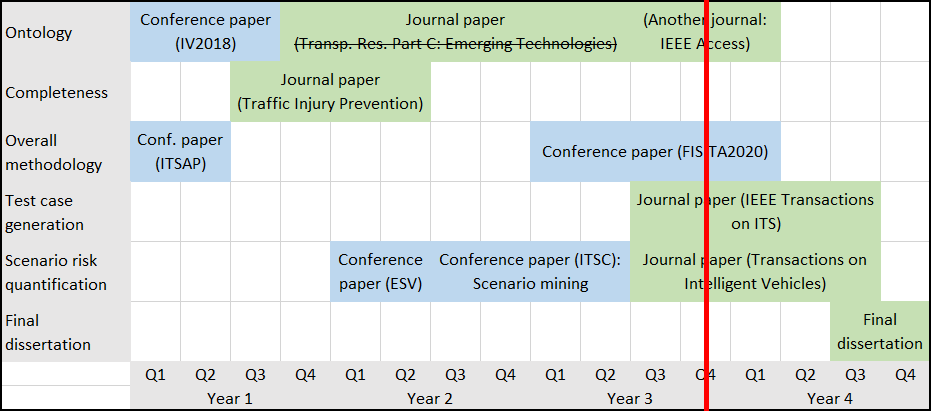
\includegraphics[width=\linewidth]{planning}
	\caption{Planning for the four main topics for which I aim to write a journal paper and the final dissertation. The red line indicates the time of writing this report.}
	\label{fig:planning}
\end{figure}

Next to the aforementioned topics, my goal is to also work on the following topics, which might result in a conference paper.
\begin{itemize}
	\item The whole methodology assumes that real-world data is being collected. Although TNO will depend on the industry to come with data, we will also collect some data ourselves. My aim would be to make part of the data we collect publicly available. I want to write a conference paper to describe the way the data is collected, the details of the data, and the potential use and limitations of the data.
	\item The traditional ISO26262 standard is used to design a system that is functionally safe. This standard is used nowadays for the development for Advanced Driver Assistance Systems. For higher levels of automation, however, this standard is not enough for designing a safe system. One issue with this standard for designing and assessing higher levels of automation is that it only allows to compute the risk of an hazardous event while the risk of a particular scenario is also very relevant. Therefore, I want to work on a paper that quantifies the risk of a scenario (which can turn into a hazardous event).
	\item The detection and classification of activities is the first step to go from the preprocessed data to the generation of test cases. I will work on this, but I do not expect to write a journal paper for this topic.
\end{itemize}

Note that scenario mining is also important, as mentioned in \cref{fig:scheme}. Because scenario mining is already addressed by other people within TNO, I did not list it above.
